\newpage\section{Instrukcja użytkowania aplikacji \NazwaSys} \label{sec:instrukcja}

\subsection{Strona główna}
\begin{figure}[h!]
\centering
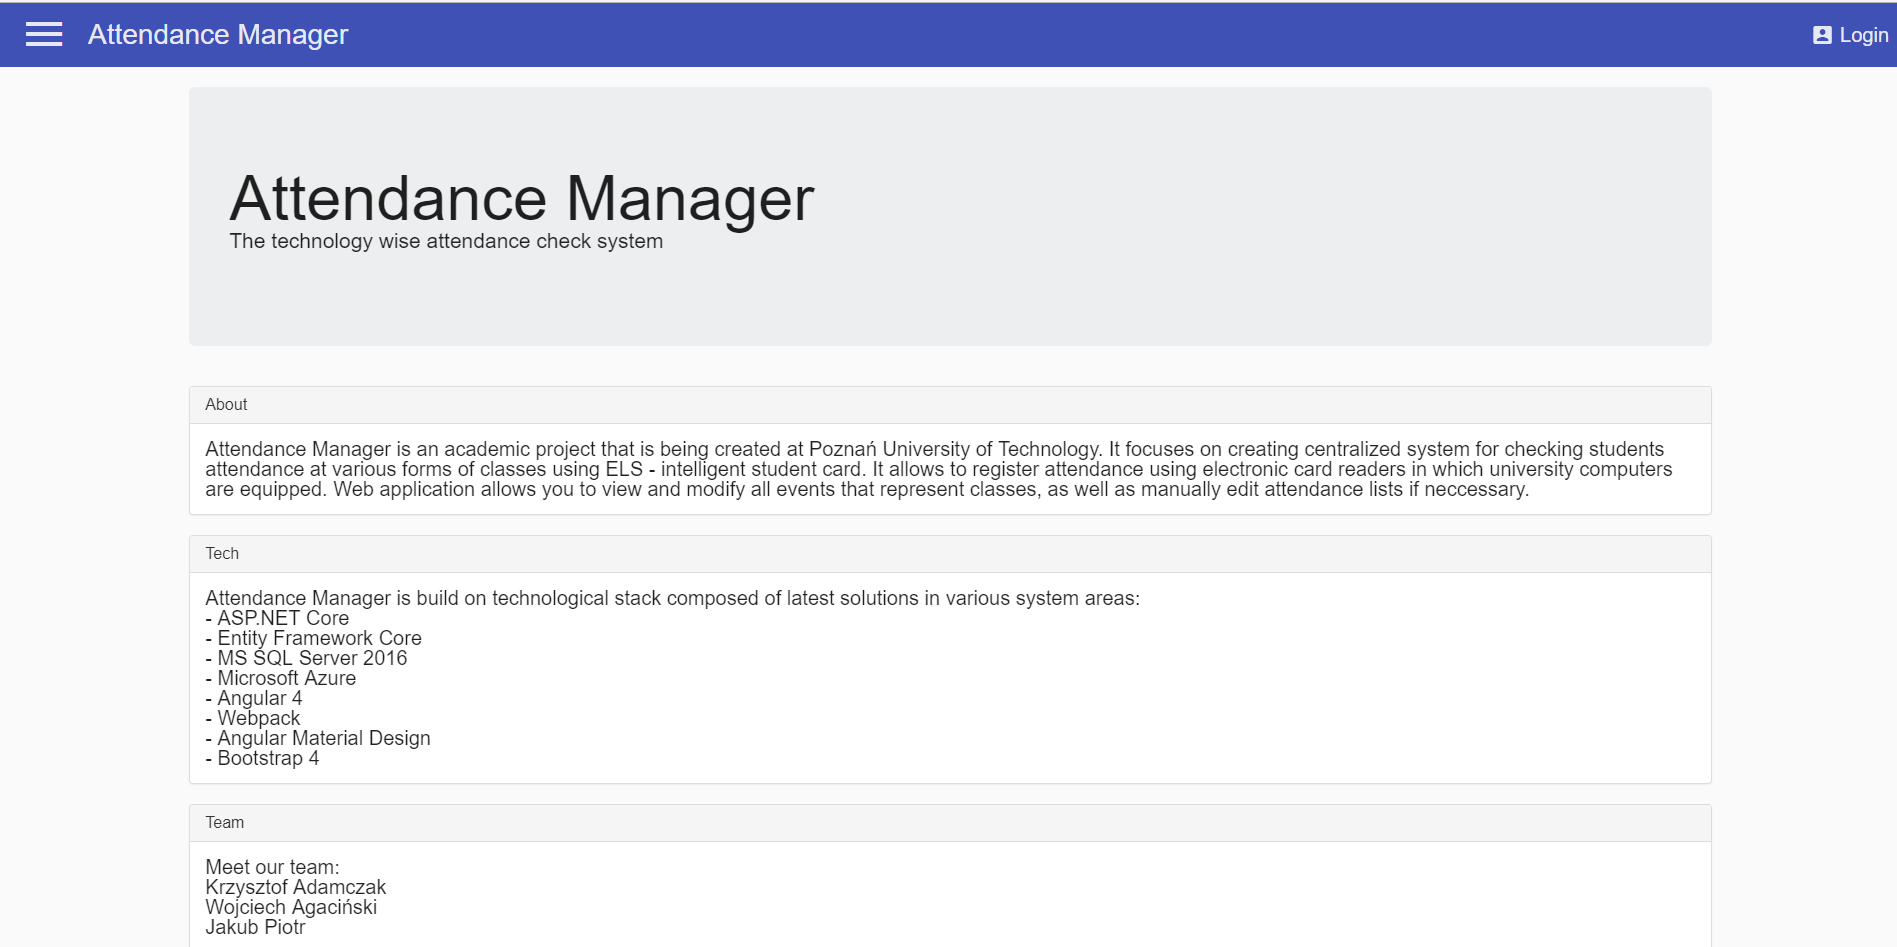
\includegraphics[height=8cm,width=15cm]{images/MainScreen}
\caption{Ekran główny aplikacji klienckiej}
\label{fig:MainScreen}
\end{figure}

Strona główna aplikacji zawiera podstawowe informacje dotyczące projektu takie jak: tytuł, opis, technologie oraz skład zespołu. W menu aplikacji po lewej stronie znajduje się przycisk otwierający menu główne aplikacji. W menu aplikacji mamy do wyboru następujące ekrany:
\begin{itemize}
    \item Home - prowadzi do strony startowej aplikacji (strony obecnej na zdjęciu)
    \item Events - strona z listą wydarzeń
    \item Add event - strona służąca do utworzenia nowego wydarzenia
\end{itemize}
\newpage
\subsection{Lista wydarzeń - Active \& Incoming}
\begin{figure}[!h]
\centering
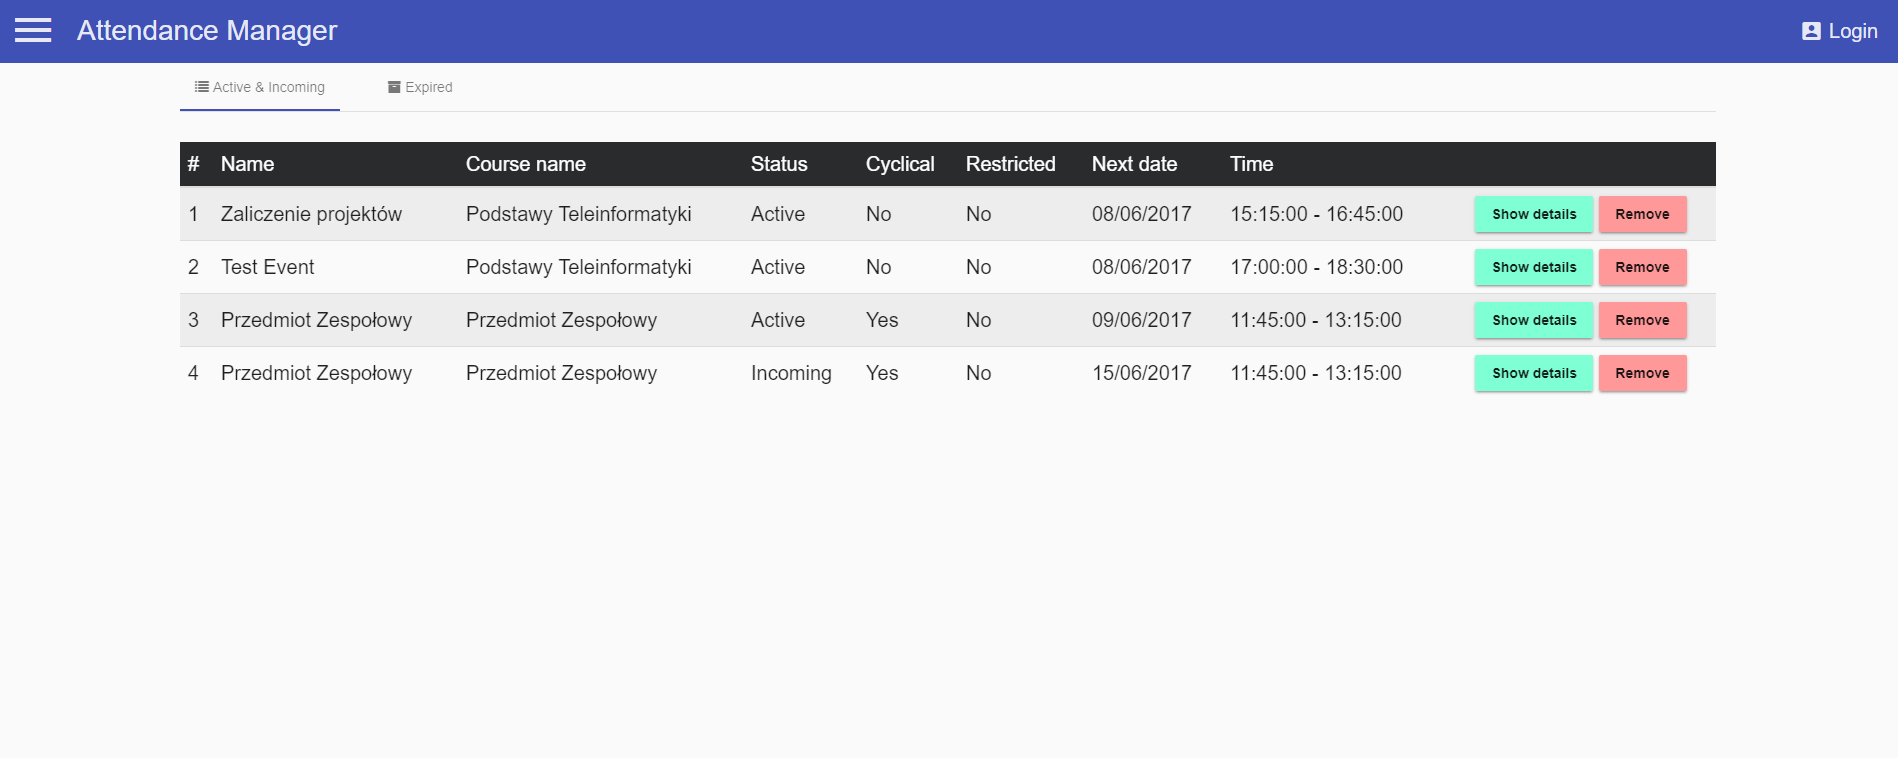
\includegraphics[height=8cm,width=15cm]{images/EventsListIncomingAndActive}
\caption{Ekran listy wydarzeń}
\label{fig:EventsListIncomingAndActive}
\end{figure}

Jest to strona zawierająca listę wydarzeń. Została ona podzielona na dwie zakładki:
\begin{itemize}
    \item Active & Incoming - zakładka zawiera tabelę z wydarzeniami nadchodzącymi oraz aktywnymi
    \item Expired - zakładka zawiera tabelę z wydarzeniami które już się wydarzyły i zakończyły
\end{itemize}
Na powyższym zdjęciu przedstawiona została zakładka `Active & Incoming`. Zawiera ona tabelę wydarzeń nadchodzących oraz aktywnych. W tabeli znajdują się pola:
\begin{itemize}
    \item Name - kolumna zawierająca nazwę wydarzenia
    \item Course name - jest to nazwa kursu do którego przypisane zostało dane wydarzenie
    \item Status - jest to obecny status wydarzenia ('Active' lub 'Incoming')
    \item Cyclical - pola informujące czy wydarzenie jest jest cykliczne
    \item Restricted - pole informujące czy wydarzenie ma ograniczoną listę uczestników mogących wziąć udział w wydarzeniu
    \item Next date - kolumna z datą wydarzenia
    \item Time - kolumna z przedziałem czasowym w którym wystąpi wydarzenie
\end{itemize}
W ostatniej kolumnie znajdują się przyciski akcji.
\begin{itemize}
    \item Show details - po wciśnięciu tego przycisku nastąpi przeniesienie na stronę zawierająca wszystkie informacje na temat wybranego wydarzenia
    \item Remove - przycisk służący usunięcie wybranego wydarzenia
\end{itemize}

\subsection{Lista wydarzeń - Expired}
\begin{figure}[h!]
\centering
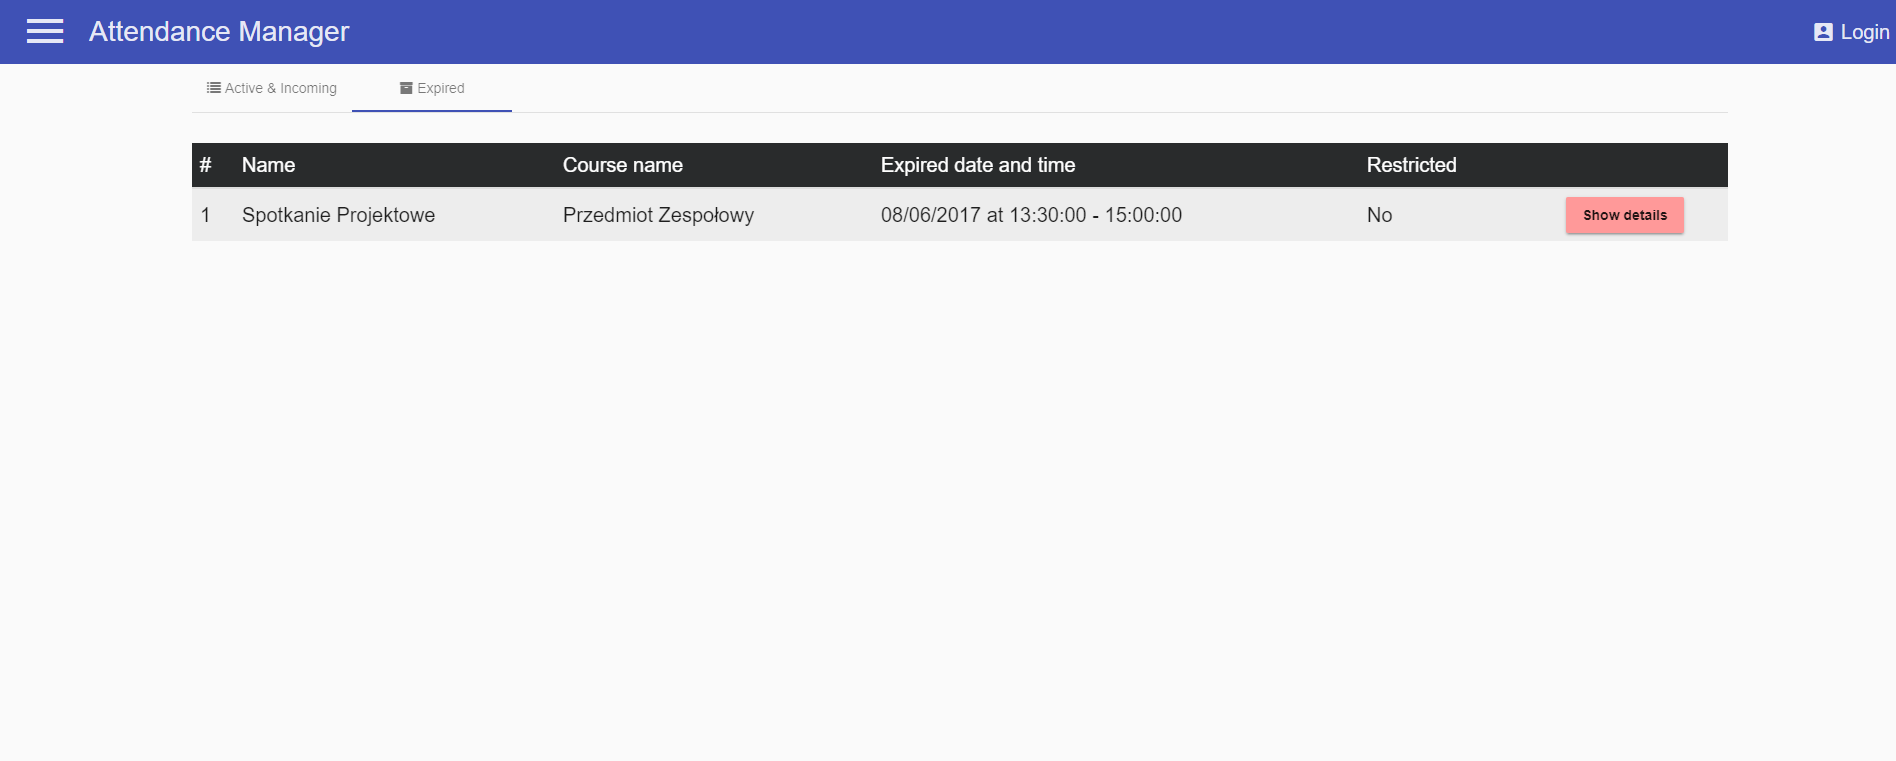
\includegraphics[height=8cm,width=15cm]{images/EventsListExpired}
\caption{Ekran listy nieaktywnych wydarzeń}
\label{fig:EventListExpired}
\end{figure}
Na powyższym zdjęciu przedstawiona została zakładka z wydarzeniami już zakończonymi. Zawiera ona tabelę z następującymi kolumnami:
\begin{itemize}
    \item Name - kolumna zawierająca nazwę wydarzenia
    \item Course name - jest to nazwa kursu do którego przypisane zostało dane wydarzenie
    \item Expired date and time - kolumna ta zawiera datę oraz przedział czasowy w którym odbyło się wydarzenie
    \item Restricted - pole informujące czy wydarzenie ma ograniczoną listę uczestników mogących wziąć udział w wydarzeniu
\end{itemize}
W tabeli znajduję się także przycisk 'Show details' który umożliwia podgląd szczegółów danego wydarzenia.

\subsection{Strona ze szczegółami wydarzenia}
\begin{figure}[h!]
\centering
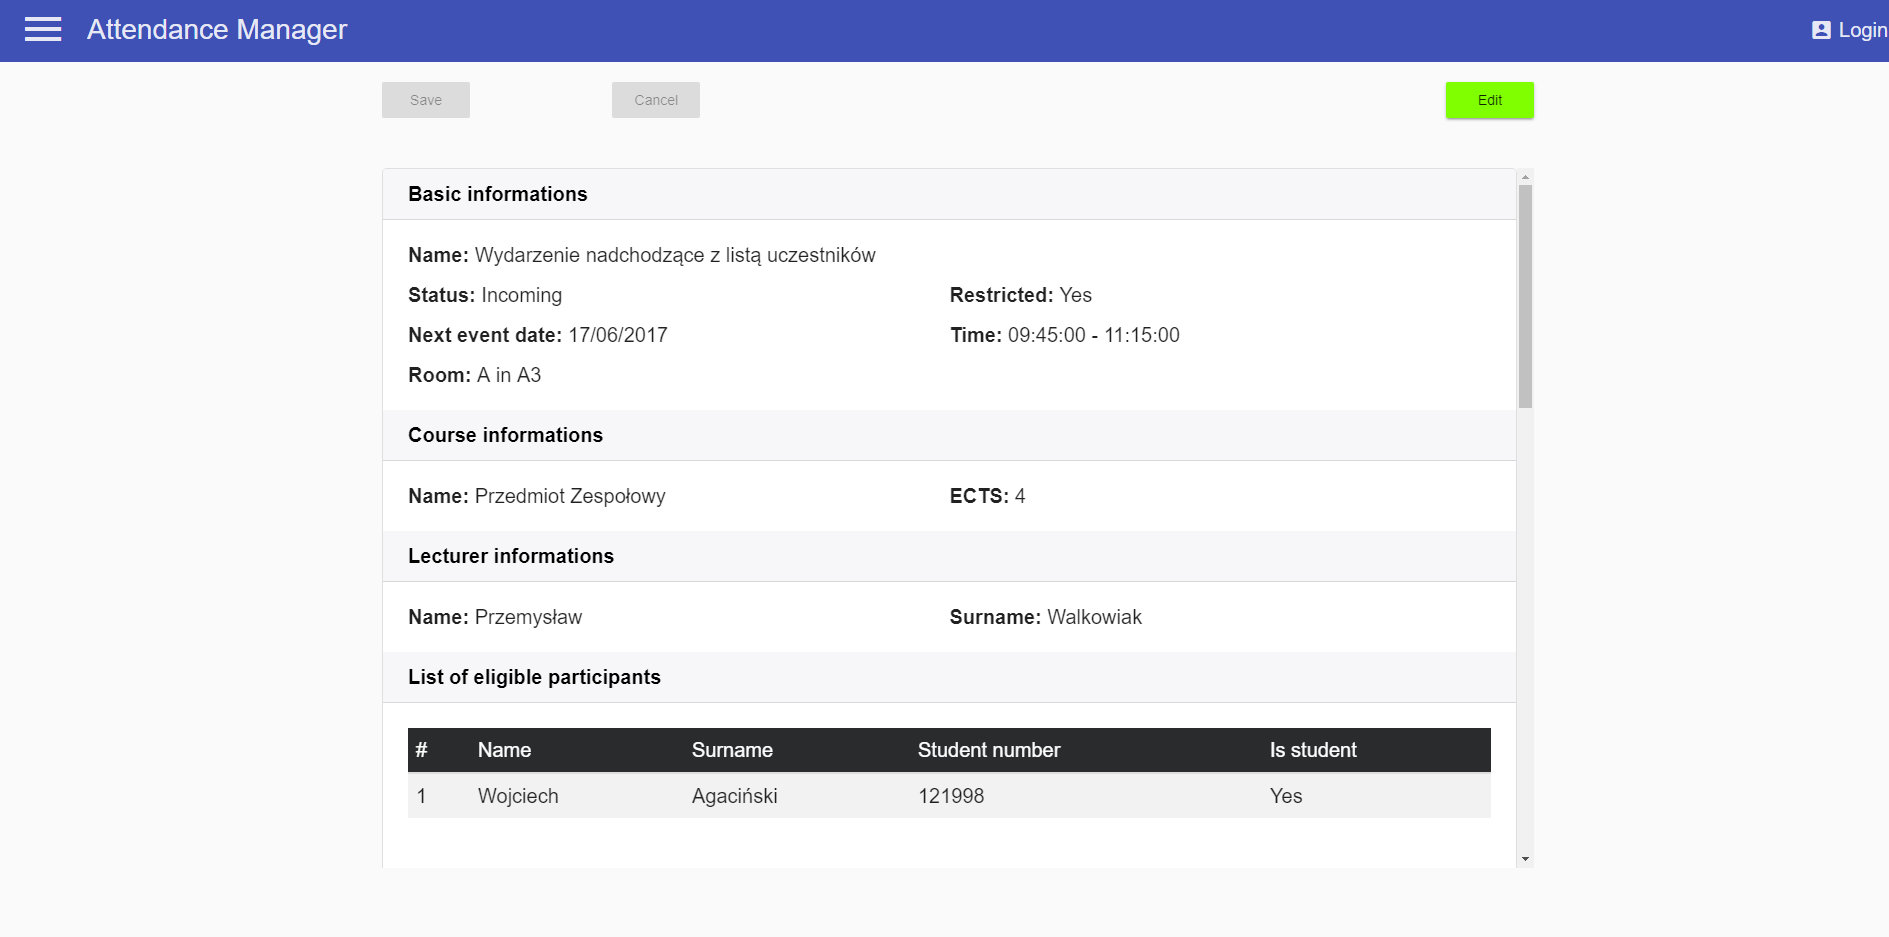
\includegraphics[height=8cm,width=15cm]{images/EventIncomingDetails}
\caption{Ekran z informacjami o nadchodzącym wydarzeniu}
\label{fig:EventIncomingDetails}
\end{figure}
Strona ta zawiera szczegółowe informacje na temat wydarzenia. Informacje zostały podzielone na sekcje:
\begin{itemize}
    \item Basic informations - sekcja zawierająca podstawowe informacje o wydarzeniu
    \item Course informations - sekcja zawierająca informację o kursie do którego podpięte jest wydarzenie. Sekcja ta jest opcjonalna. W przypadku braku podpietego kursu sekcja ta nie zostanie wyświetlona
    \item Lecturer informations - sekcja zawierająca informację o przypisanym do wydarzenia wykładowcy
    \item List of eligible participants - w przypadku gdy wydarzenie jest zamknięte (posiada listę uczestników uprawnionych do wzięcia udziału w wydarzeniu) pojawia się sekcja z listą uprawnionych uczestników
    \item Attendance list - sekcja zawierająca listę obecności. Pojawia się w przypadku gdy event jest aktywny lub zakończony
\end{itemize}
Na tej stronie możliwa jest edycja wydarzenia. W zależności od statusu wydarzenia niektóre pola/sekcje mogą być niedostępne do edytowania.
\begin{itemize}
    \item Wydarzenie nadchodzące - możliwa jest edycja prawie wszystkich pól oprócz listy obecności
    \item Wydarzenie aktywne - możliwa jest edycja jedynie listy obecności
    \item Wydarzenie zakończone - możliwa jest edycja jedynie listy obecności
\end{itemize}

\subsection{Tworzenie nowego wydarzenia}
\begin{figure}[h!]
\centering
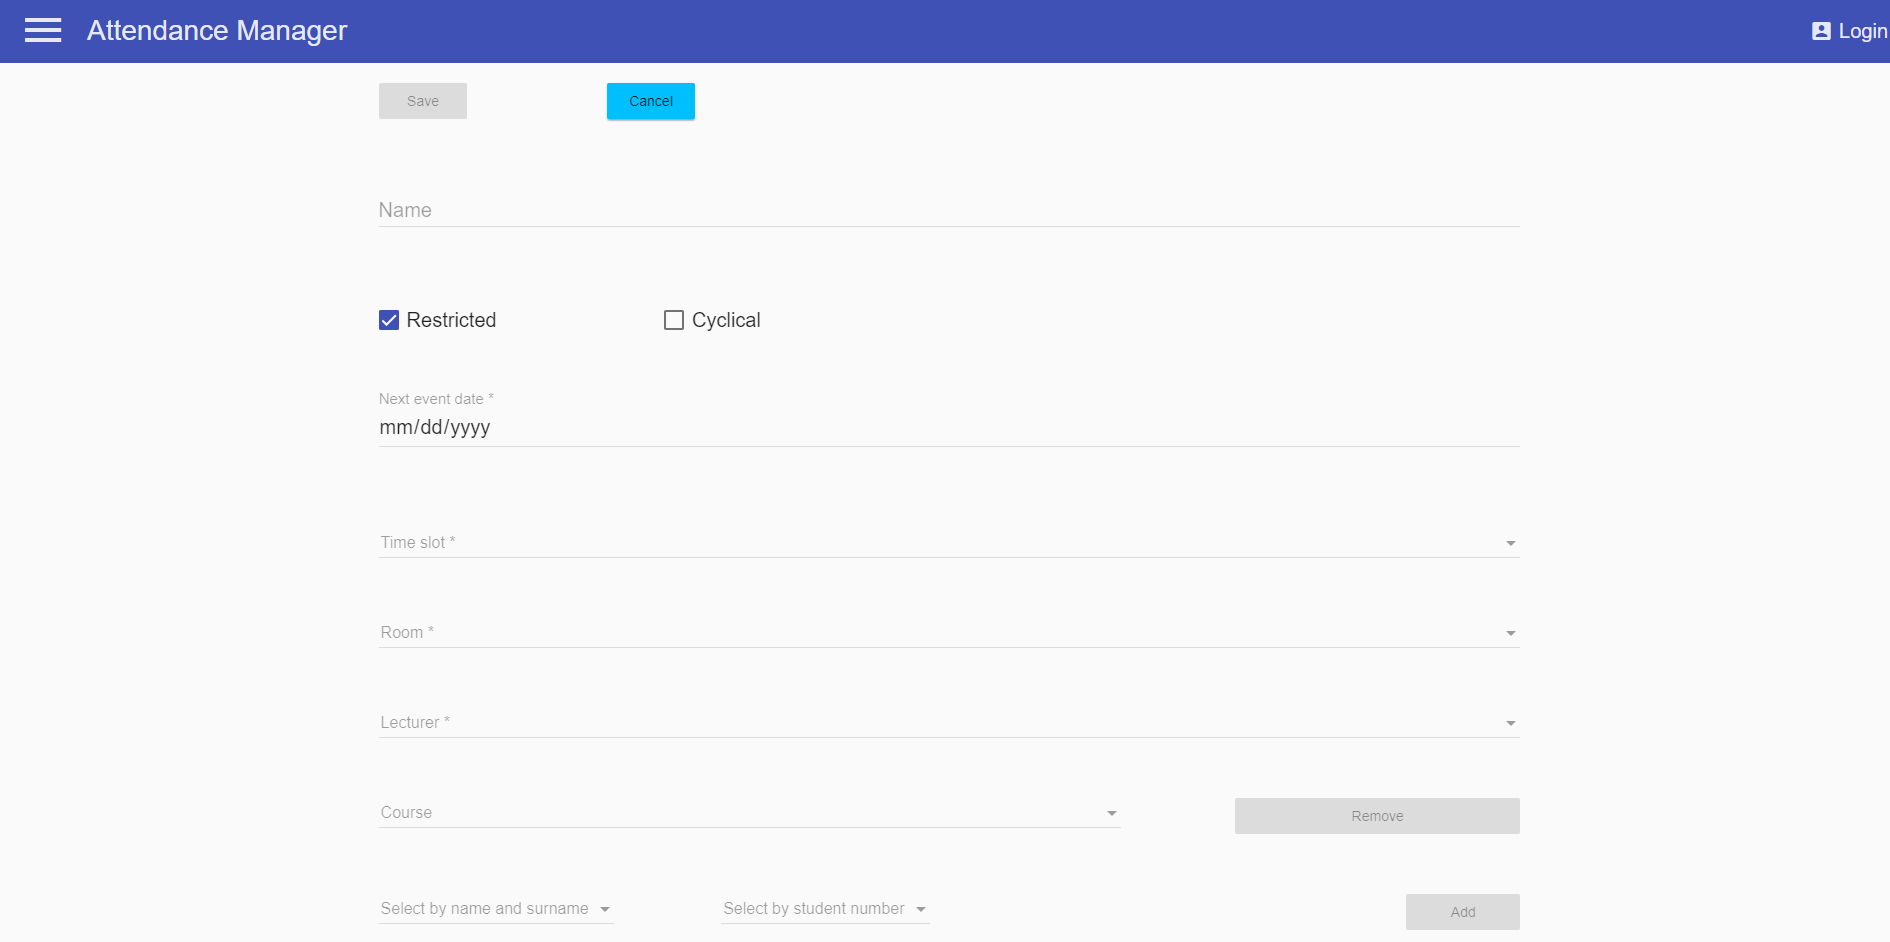
\includegraphics[height=8cm,width=15cm]{images/AddNewEvent}
\caption{Ekran dodawania nowego wydarzenia}
\label{fig:AddnewEvent}
\end{figure}
Jest to strona służąca dodawaniu nowych wydarzeń. Zawiera ona formularz z odpowiednimi polami. Pola wymagane zostały odpowiednio oznaczone. Możliwość dodawania listy uczestników odblokowuje się po wybraniu opcji 'Restricted'.